\section{Versuchsaufbau und Durchführung}
\label{sec:experimental_setup_and_conduction}
Dieses Experiment soll die Funktionsweise der szintillierenden Fasern in dem LHCb-Detektor beschreiben. 
Der Versuchsaufbau besteht aus drei zentralen Komponenten.
Einer szintillierenden Faser,
einer LED als Lichtquelle sowie einem Spektrometer,
am Ende der Faserzur Lichtdetektion. 
Die LED ist horizontal entlang der Faser verschiebbar, 
sodass die Faser an verschiedenen Positionen angeregt werden kann.
Das Spektrometer ist an einem motorisierten Halter befestigt, 
der eine Positionierung unter verschiedenen horizontalen und vertikalen Winkeln relativ zum Faserende ermöglicht. 
Sowohl die Motoren als auch die LED und das Spektrometer werden über eine dedizierte Steuersoftware geregelt.
Ein Foto des gesamten Aufbaus ist in der \autoref{fig:setup} dargestellt.
\begin{figure}
    \centering
    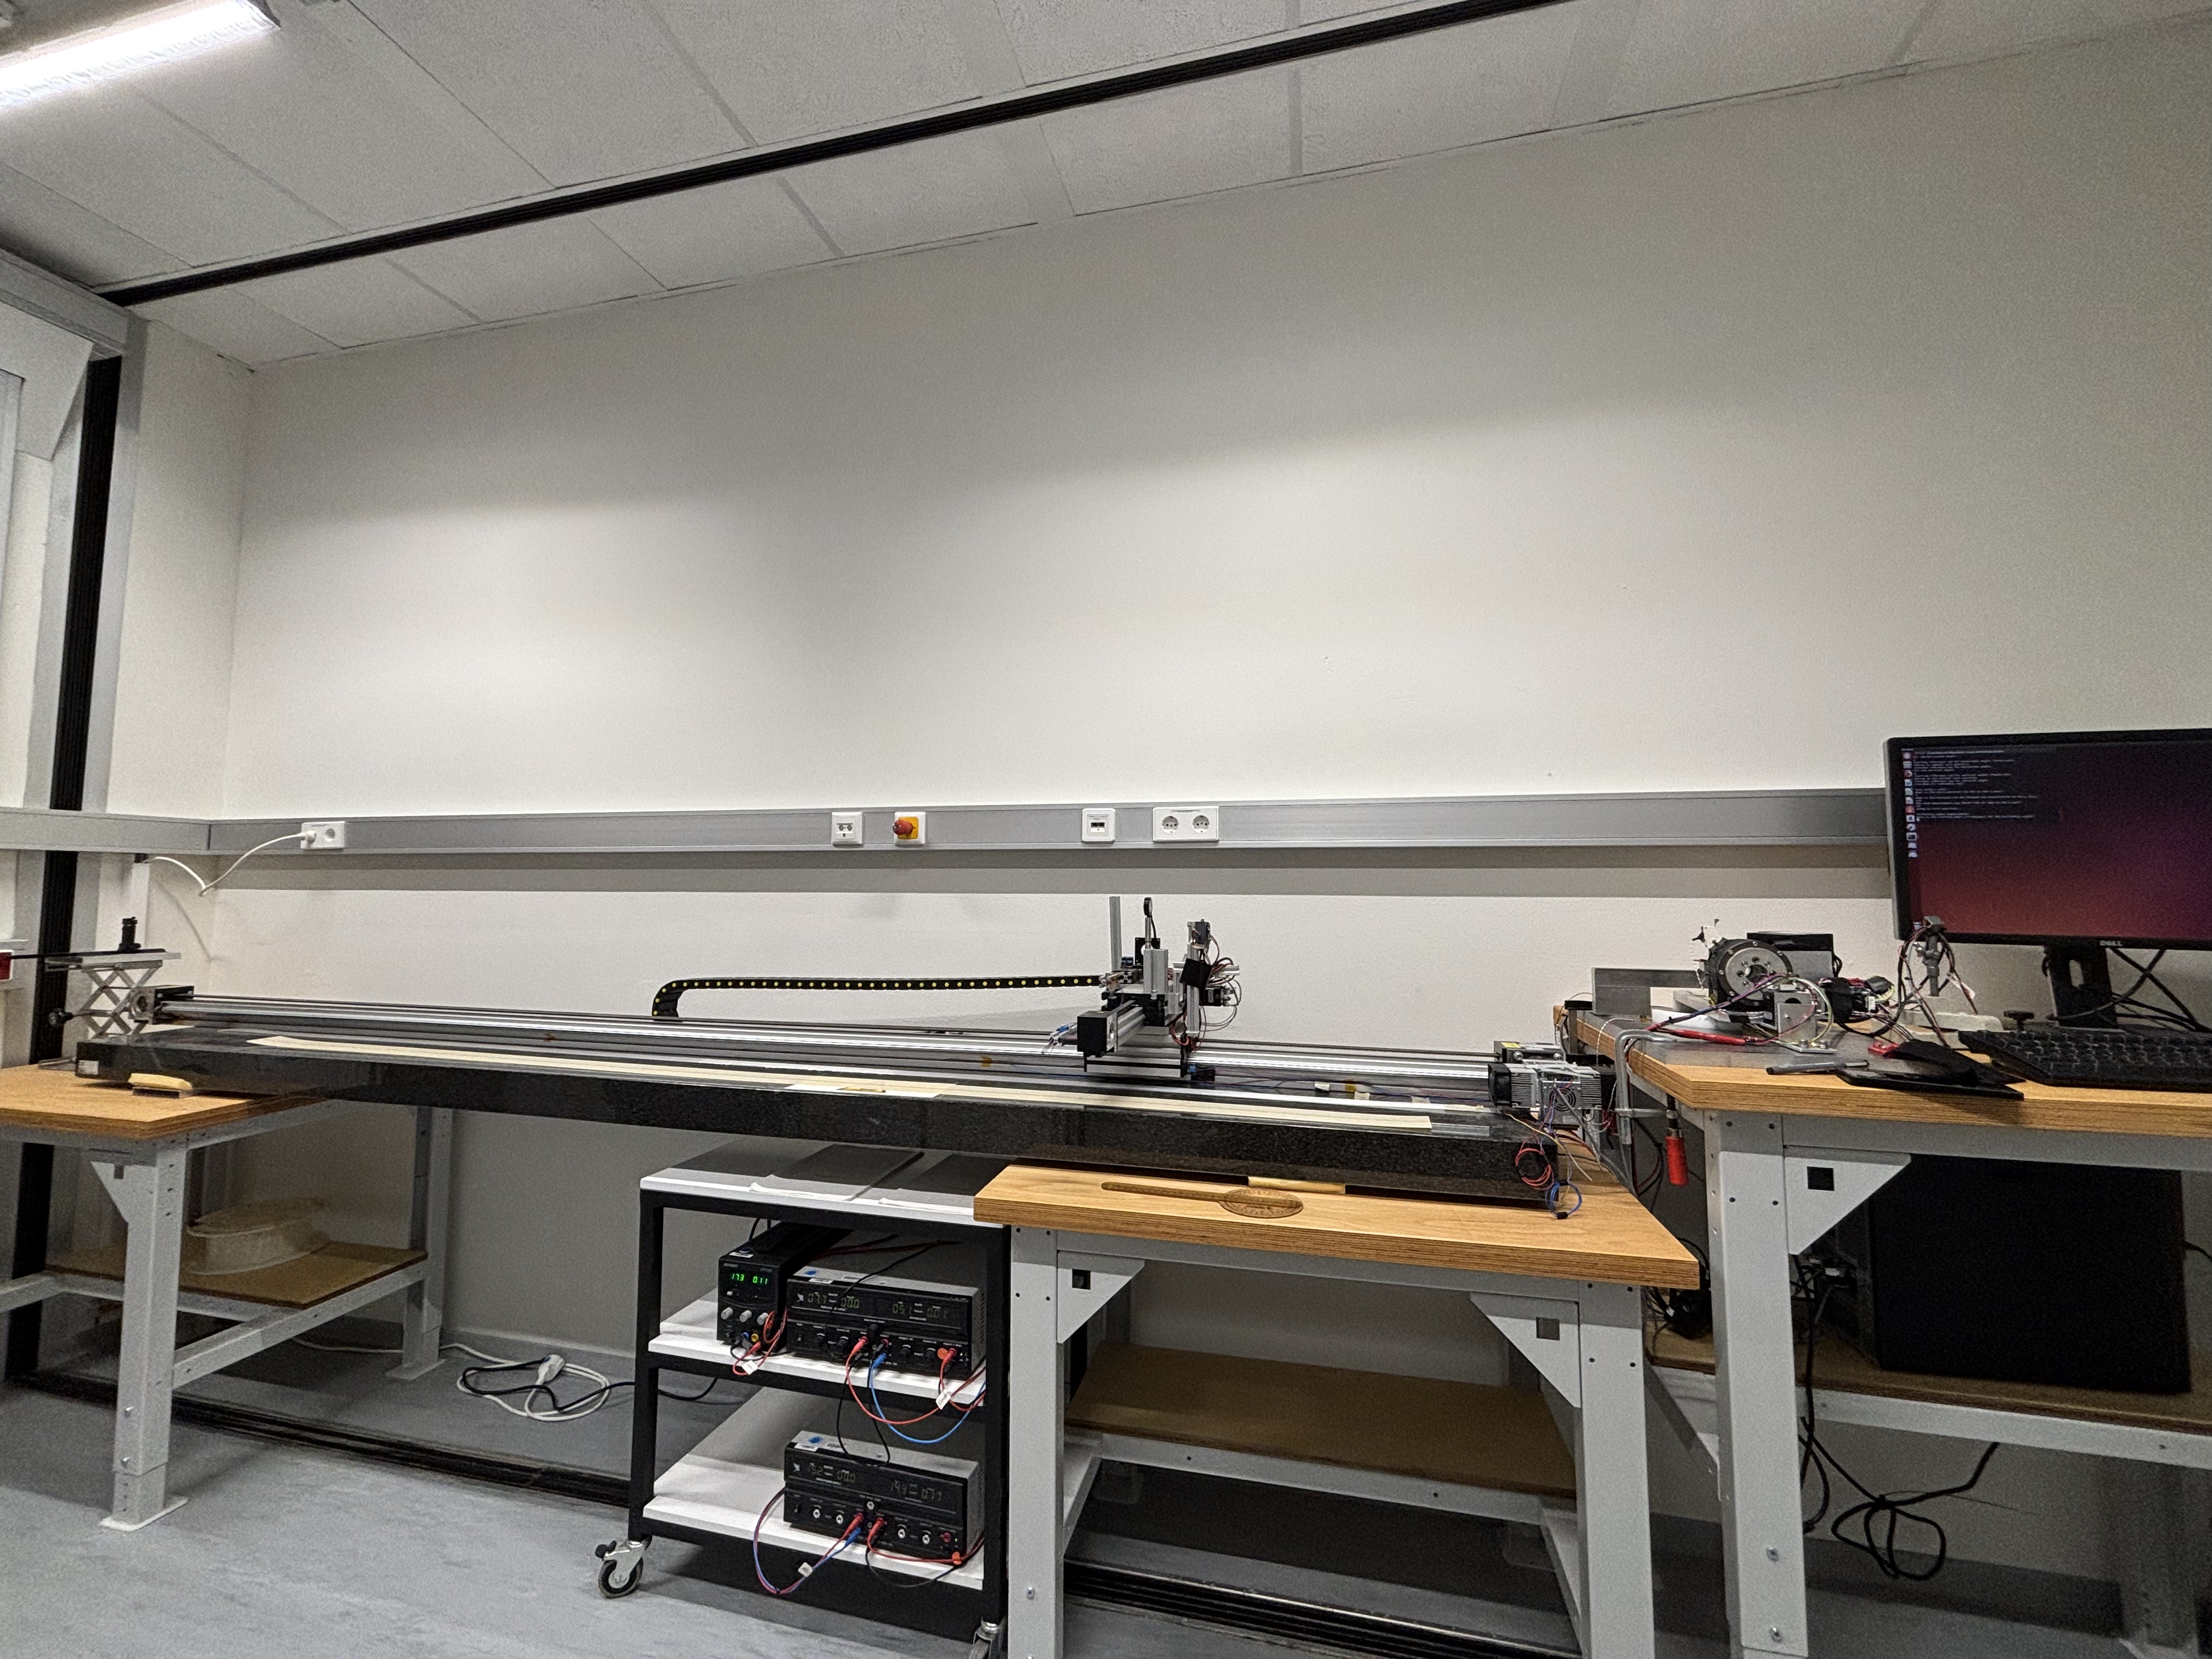
\includegraphics[width=10cm, keepaspectratio]{content/Figures/gesamt.png}
    \caption{Aufbau einer szintillierenden Faser mit einer Photodiode und einem Spektrometer.}
    \label{fig:setup}
 \end{figure}
 \subsection{Versuchsdurchführung}
\label{sec:versuchsdurchführung}

Zunächst wird ein Referenzspektrum aufgenommen, um das Hintergundspektrum im Versuchsraum zu charakterisieren.
Die Messung wird dafür bei einem kleinen Winkel relativ zur Faserachse durchgeführt und sowohl mit eingeschaltetem Raumlicht als auch mit ausgeschaltetem Raumlicht wiederholt. 

Um die radiale Symmetrie der Lichtintensität am Faserende zu überprüfen, 
wird die Intensität bei fester Anregungsposition durch die LED für ein zweidimensionales Raster von Winkelpaaren gemessen. 
Der horizontale Winkel wird dabei im Bereich von $-18°$ bis $30°$ variiert,
der vertikale Winkel im Bereich von $-6°$ bis $35°$.

Abschließend wird die Intensität am Faserende für verschiedene Anregungspositionen der LED entlang der Faser gemessen.
Dafür wird bei einem festen horizontalen Winkel von $10°$ 
und einem variablen vertikalen Winkel von $0°$ bis $40°$ bei verschiedenen Anregungspositionen der LED entlang der Faser gemessen.
Gemessen wird an zehn verschiedenen Anregungspositionen entlang der Faser.